\subsection{Long-range number-units}
To successfully perform the NA-task, the LSTM network should encode and store the grammatical number of the subject up to one step before the verb, when prediction of the verb form (singular or plural) occurs. In some cases, this may be quite challenging, in particular in the case of a long-range dependency between subject and verb, and when another noun with an opposite number appears before the verb (cite and cite). This section explores the underlying mechanism that enables the network to encode and store number information in various syntactic constructions, including those with such interfering nouns. The section has the following structure: subsection 5.1.1 describes an ablation study, which reveals \textit{long-range number units (LR-number units)} that can store and carry number information from subject to verb across interfering noun. Then, subsection 5.1.2 describes in details the gating and state dynamics of the identified LR-number units during the processing of sentences with long-range dependencies. Finally, subsection 5.1.4 explores the structure of the efferent weights of LR-number units that project onto the output layer.

\subsubsection{Local vs. distributed code - an ablation study}
Generally, number information may be stored in the network in either a local, sparse, or a distributed way, depending on the fraction of active units that carry this information. We hypothesized that if the network uses a local or sparse coding, meaning that there's a small set of units that encode number information, then ablating these units would lead to a drastic decrease in performance on the NA-task, compared to when ablating other units. To test this, we conducted ablation experiments in which each time a single unit of the network is ablated and the resulting model is then evaluated on several NA-tasks. Each NA-task contained sentences with a fixed syntactic structure, such as "Det Noun Adv Verb" or "Det Noun P Det Noun Verb", and each task was composed of several conditions depending on the possible assignments of grammatical number to the nonu(s) in the sentence. In addition, we also evaluated each ablated model on the Linzen task (see section 3.1 for details about all NA-tasks). Tables 1 summarizes the results of all ablation experiments, showing units whose ablation resulted in a performance decrease of more than 10\% (TODO: choose a non-arbitrary threshold by looking at the distribution across all experiments - mean + 3sd for example). For each NA-task, the performance of the full, non-ablated, model is also reported.


\begin{center}
\begin{table}[ht]
\begin{tabular}{|P{1.4cm}|P{0.4cm}||P{0.6cm}|P{0.6cm}|P{0.6cm}|P{0.6cm}|P{0.6cm}|P{0.6cm}|P{0.6cm}|P{0.6cm}|P{0.6cm}|P{0.6cm}|P{0.6cm}|P{0.6cm}||P{0.6cm}|}
\hline
\B NA task & \B C & \B \textcolor{blue}{770} & \B \textcolor{blue}{776} & \B \textcolor{red}{988} & \B \textcolor{red}{1283} & \B Full \\
\hline
\hline

% Singular condition

\B Simple & \B S & - &  - &    - &  - &  100 \\

\B Adv & \B S &  - &  - &  - &  - &  100 \\

\B 2Adv & \B S &  - &  - &  - &  - &  99.8 \\

\B Co-Adv & \B S &  - &  - &  \textcolor{red}{84.0} &  \textcolor{red}{84.0} &  98.8 \\

\B namePP & \B S &  - &  - &  - &  - &  98.9 \\

\B nounPP & \B SS &  - &  - & - &  - &  97.5 \\

\B nounPP & \B SP &  \B - &  - &  \textcolor{red}{58.8} &  - &  88.5 \\

\B subjrel & \B SS &   - &  - & \textcolor{red}{88.0} &  - &  97.0 \\

\B subjrel & \B SP &  \B - &  - &  - &  - &  58.8 \\

\B objrel & \B SS & \B - &  - &  - &  - &  64.7 \\

\B objrel & \B SP &  \B - &  - &  - &  - &  45.7 \\

\hline
% % Plural condition
\B Simple & \B P &  - &  - &  - &  - &  100 \\

\B Adv & \B P &  - &  - &  - &  - &  99.6 \\

\B 2Adv & \B P & - &  - & - & - &  99 \\

\B Co-Adv & \B P &  - &  \textcolor{blue}{78.9} & - &  - &  99.7 \\

\B namePP & \B P & - &  \textcolor{blue}{57.6} &  - &  - &  66.8 \\

\B nounPP & \B PS &  \textcolor{blue}{85.2} &  \textcolor{blue}{49.7} & - &  - &  93.2 \\

\B nounPP & \B PP &  - &  \textcolor{blue}{81.7} &  - &  - &  98.3 \\

\B subjrel & \B PS &  \textcolor{blue}{85.8}  &  \textcolor{blue}{58.6}  &  - &  - &  87.8 \\

\B subjrel & \B PP &  - &  \textcolor{blue}{88.1} &  - &  - &  99.3 \\

\B objrel & \B PS & - &  - &  - &  - &  69.0 \\

\B objrel & \B PP &  - &  - &  - &  - &  81.0 \\
\hline
\hline
\B Linzen & \B - &  ? &  ? &  ? &  ? &  ? \\
\hline
\end{tabular}
\caption{Ablation experiments results: Percentage of correct subject-verb agreements in all NA-tasks (section 3.1). Full - non-ablated model, C - condition, S - singular, P - plural. For task with two nouns, SS - singular-singular, SP - singular-plural, PS - plural-singular, PP - plural-plural. Red: singluar number units, Blue: Plural number units.}
\end{table}
\end{center}

We first highlight several aspects in the behavioral results of the full network (table 1 - right column), before looking into the ablation results. First, some NA-tasks and conditions are clearly more difficult for the network than others. For example, performance on the simple NA-task is better than that on the nounPP NA-task, which in turn is better than that of the objrel task. This matches previoulsy reported results for humans and LSTM-LMs (cite and cite). Second, having a distracting second noun before the verb, with an opposite number than the first one, is clearly a more challenging case for the network. For the nounPP, subjrel and objrel tasks, performance on the SP and PS conditions was lower than that on the SS and PP conditions. We get back to this point in section 5.4. Finally, singular information of the first noun was in most cases more difficult to be reliably encoded for long-range dependencies compared to plural. For example, in all above tasks, performance on condition SS was lower than PP, and that of SP lower than PS. Interestingly, this singular-plural asymmetry was already reported in humans (cite Bock). However, in contrast to phonological or morphological-based explanations suggested in this study, our results point to a cause residing at the word level, given that the language model was trained on word tokens.

We next highlight several important aspects in the ablation-experiment results. First, in all NA-tasks, only four units from the entire network (1300 LSTM units in total) had a significant effect on task performance. This result suggests a local coding scheme for long-range grammatical-number information (TODO: quantify a 'significant' reduction). Second, we note that all number units emerged at the second layer of the network. This seems appropriate if number information needs to be directly projected to the output layer for correct verb-form prediction (?what about a network with a single layer of 1300 units?). In section 5.1.4 we further explore these projection weights from number units. Third, for simple, 1Adv and 2Adv NA-tasks, none of the units had a significant effect on task performance. This suggests that for short-range dependencies number information may be encoded elsewhere in the network, perhaps via a more distributed code. (TODO: identify the short-range number units from the resulting weights of the classifier in the generalization-across-time experiment). We therefore make the distinction between long-range (LR) and short-range (SR) number units in the network. We return to this point in section 5.1.4. Fourth, LR-number units can be further divided into two types, depending on the grammatical number of the first noun in the sentence. Units 770 and 776 had a significant effect only when the first noun was plural, but not singular, and vice versa for units 988 and 1283 (blue and red in table 1, respectively). We therefore refer to the former as \textit{LR-plural-number units} and to the latter \textit{LR-singular-number units}. Finally, we note that two of the number units - unit 770 and 988 - had a tremendous effect on network performance in both nounPP-SP\&PS conditions. These two conditions are in particular revealing since they involve both a long-range dependecy (over a prepositional phrase) and an interferring noun before the verb, while performance of the non-ablated network is relatively high (88.5\%\&93.2\%, respectively) compared to similar conditions in the subjrel and objrel tasks. Ablating one of these two units brought the network from high performance on the NA-task to around chance-level performance (58.8\%\&49.7\%, respectively). Also, compared to the other two number units (770\&1283) their effect was observed in a larger number of conditions. In the next subsection, we will therefore focus on these two units.

\subsubsection{Visualizing unit dynamics}
Results from the ablation study suggest that there's a small set of units that encodes number information for long-range dependencies, in particular, we find that in some conditions two units can bring the network from relatively high performance to around chance-level performance on the NA-task (section 5.1.1). However, it remains unclear what is the underlying mechanism required for this task. Specifically, in conditions nounpp-SP\&PS discussed above - how exactly the two number units 776 \& 988 successfully carry grammatical-number information across the prepositional phrase albeit an interferring noun before the verb? To better under thing, this section looks into gate and state dynamics of these units during the processing of sentences from the nounPP NA-task. 

To anticpate the results and facilitate their interpreations, we begin by discussing what one would hypothesize about the gate and state dynamics of an LSTM number unit that are required for solving the NA-task. We recall that the update rule of the LSTM cell has two terms (equation 1.4). In the first term $f_t * C_{t-1}$, the forget gate controls whether to keep the previous content $C_{t-1}$ stored in the cell ($f_t=1$ means perfect remembering) or forget it ($f_t=0$ - complete forgetting). In the second term $i_t*\tilde{C_t}$, the input gate controls whether the information currently presented to the network could be updated into the cell state: $i_t=1$ - full access, $i_t=0$ - no access. Therefore, to produce a correct number agreement, it seems that a number unit should at least exhibit the following two dynamics: (1) To allow a new cell content $\tilde{C_t_{subject}}$, presumably containing the grammatical number of the current subject (TODO: show it spearately from the input gate, by plotting $\tilde{C}$ values of singular and plural nouns), update onto the cell variable, the input gate should open ($i_t_{subject}$~=1) at time $t=t_{subject}$. In addition, to prevent interferring information such as an opposite grammatical number of a following noun, updating onto the cell, the input gate should be closed ($i_t=0$) during all successibe time steps until the verb; (2) To successfully strore the number information in the cell state for a long-range dependency, the forget gate should be in a remembering state ($f_t=1$), starting one step after the subject. Figure 1B summarizes these two requirements.  

Figure 2 shows the actual gate and state dynamics of units 776 and 988 during the processing of sentences from the nounPP NA-task. For each unit, we draw the cell state, forget-gate and input-gate activity (panels A-C, respectively), and for each of these cases, the four condition (SS, SP, PS and PP) are described in separate curves. Error-bars represent standard deviation across 1000 sentences in each condition.

\begin{figure}[h!]
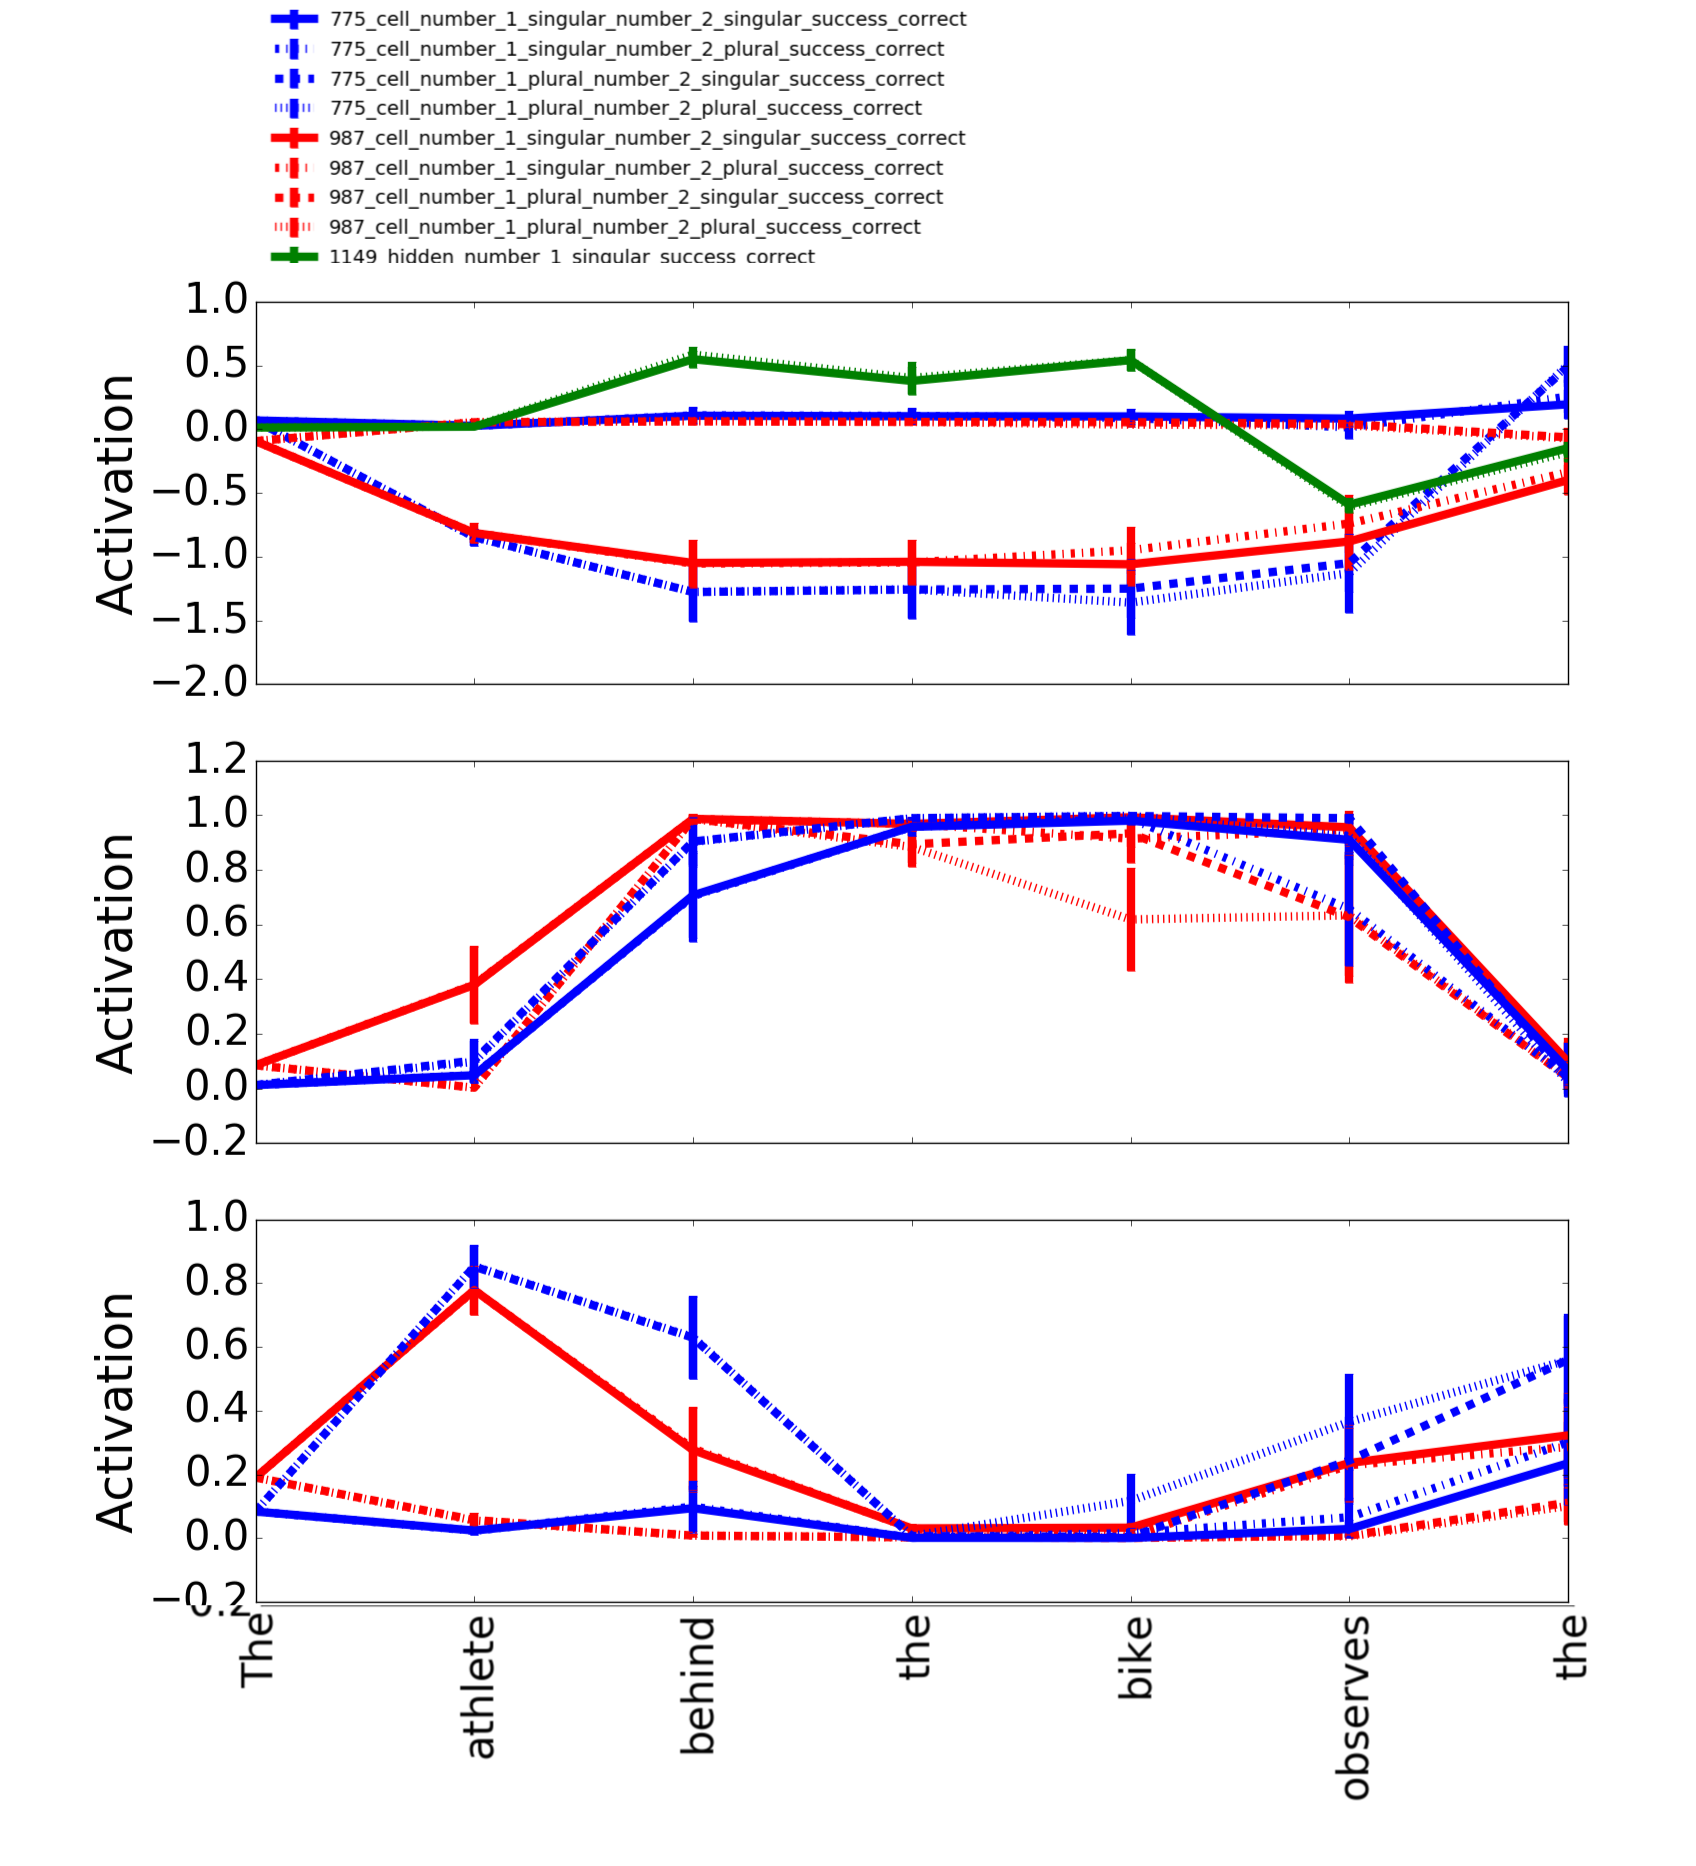
\includegraphics[width=\linewidth]{Figures/Figure2_number_units.png}
\caption{Cell and gate activations during processing of a sentence with a prepositional phrase between subject and verb. (A) Cell activity $C_t$ for the two number units 775 and 987 and output activity $h_t$ for the syntax unit 1149, for all four combinations of grammatical numbers of the two nouns. Note that the cell activity of units 775/987 is non-zero only when the first noun is plural/singular, respectively. (B) Corresponding forget-gate activity for the same number units. Note that gate activity is indifferent of the grammatical number of both nouns and that its value is close to one during the PP until after the verb. (C) Input-gate activity of the same units. Note that the gate value of unit 775/987 spikes around the first noun only when it is plural/singular.}
\end{figure}

Input-gate dynamics of both number units seem to indeed correspond to the first requirement described above. Input-gate activity spikes around the subject and stays close to zero until the verb. One difference with the description above is the non-zero activity of the input gate at the time step immediately following the subject. This may be due to several reasons that requires further research. One possible explanation for this is that the network has developed this behavior as a heuristic to deal with compund nouns, given that an interferring noun could immediately follow the subject, whereas for compound nouns the important number information resides at the second noun (TODO: discuss this part in the meeting. Perhaps we could easily check this in an experiment.). Importantly, the input gate of unit 988 is open only when the subject is singular, and that of unit 776 is open only when the subject is plural. This is in accordance with the results of the ablation study, supporting the labeling of 988 and 776 as singular and plural units, respectively. 

Forget-gate dynamics of both number units seem too to follow the requirements described above. Forget-gate activity of both units goes abruptly towards value of one at the time step following the subject, and stabely stays at this level until the verb. Note also that the forget-gate exhibits the same dynamics indifferently to the grammatical number of the subject - for all four conditions (SS, SP, PS and PP), its activity is approximately the same. This seems appropriate for the following two reasons. First, the network cannot know in advance whether an interferring noun will appear. This seems to explain why gate activity should be the same for SS and SP, or PP and PS. This can be thought of as \textit{just in case} number encoding - once the network has encountered a subject, its number is stored in the cell state of a number unit "just in case" an interferring noun will later appear. Second, when the subject is plural, the singular unit 988 should not output any signal to the output layer, otherwise it may interfere with the correct prediction of the verb form. It is therefore important to ensure that the cell value is different than in the case of a singular subject. This seems to explain why the gate activity of unit 987 is the same whether the first noun is singular or plural, that is, why gate dynamics for condition SS and SP is similar to that of PS and PP. And the same hold for gate dyanmics of unit 776. Last, we note that the forget-gate activity resets towards zero, one step after the verb. At this point, number information of the subject is not useful anymore, and the cell variable is free to encode new number information. 
 
Finally, cell-state activity should reflect the dynamics of the input and forget gates. Figure 3C shows the cell values of the number units for all four conditions. Indeed, cell value becomes non-zero at $t_{subject}$ and preserves this value until the verb only for the relevant conditions. For conditions SS and SP, unit 987 encodes singular as $C_t ~= -1$ and is approximately zero during sentence processing in the other two conditions (PP and PS). Similarly, unit 776 encodes plural with a non-zero, negative, value only in the relevant conditions (PP and PS) but not in the other two (SS and SP).

To summarize, it is therefore seem clear why ablating either one of these two units brings the network close to chance level on the nounPP task - without these units that store and remember the grammatical number of the subject in their cell variable, the network hopelessly tries to solve the task.

TODO: change the order of the panels in Figure 2. Input, gate and then cell. 

\subsection{Short-range number units}
\lipsum[1]

\begin{figure}
\centering
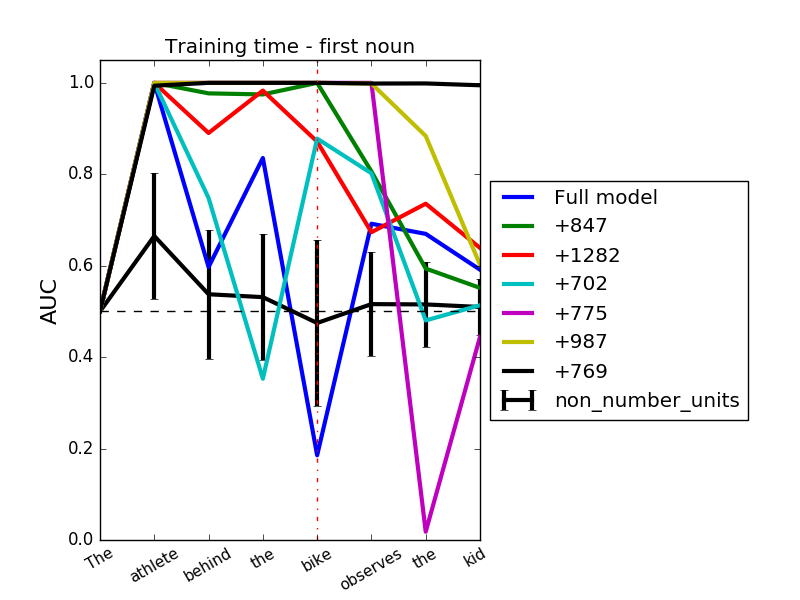
\includegraphics[width=\linewidth]{Figures/Figure3_number_units_GAT.png}
\caption{Generalization across time. To test whether the grammatical number of the first noun can be decoded from units activity at different time points, a linear-SVM was trained on unit activations $h_t$ at the time step of the first noun and then evaluated on all other time points. Area Under of Curve (AUC) values are shown for several cases: decoding from all LSTM units (full-model, black), a single number unit (775, purple; 1282, red...), average across all non-number units (black, error-bars represent standard-deviation). Note that the decoding of first-noun number is significantly higher from number units compared to all other units ($p-value<0.$).}
\end{figure}


\subsubsection{Predicting the verb form}
Output weights + PCA
Section 5.1.2 summarizes these findings. Finally, to predict the proper verb form, number information should be projected from number units to the output layer. Section 5.1.3 explores the structure of the efferent weights of the number units. 

These efferent weights propagate grammatical-number information to the output layer, allowing for the prediction of the proper verb form (singular or plural). 

\begin{figure*}[t]
\centering
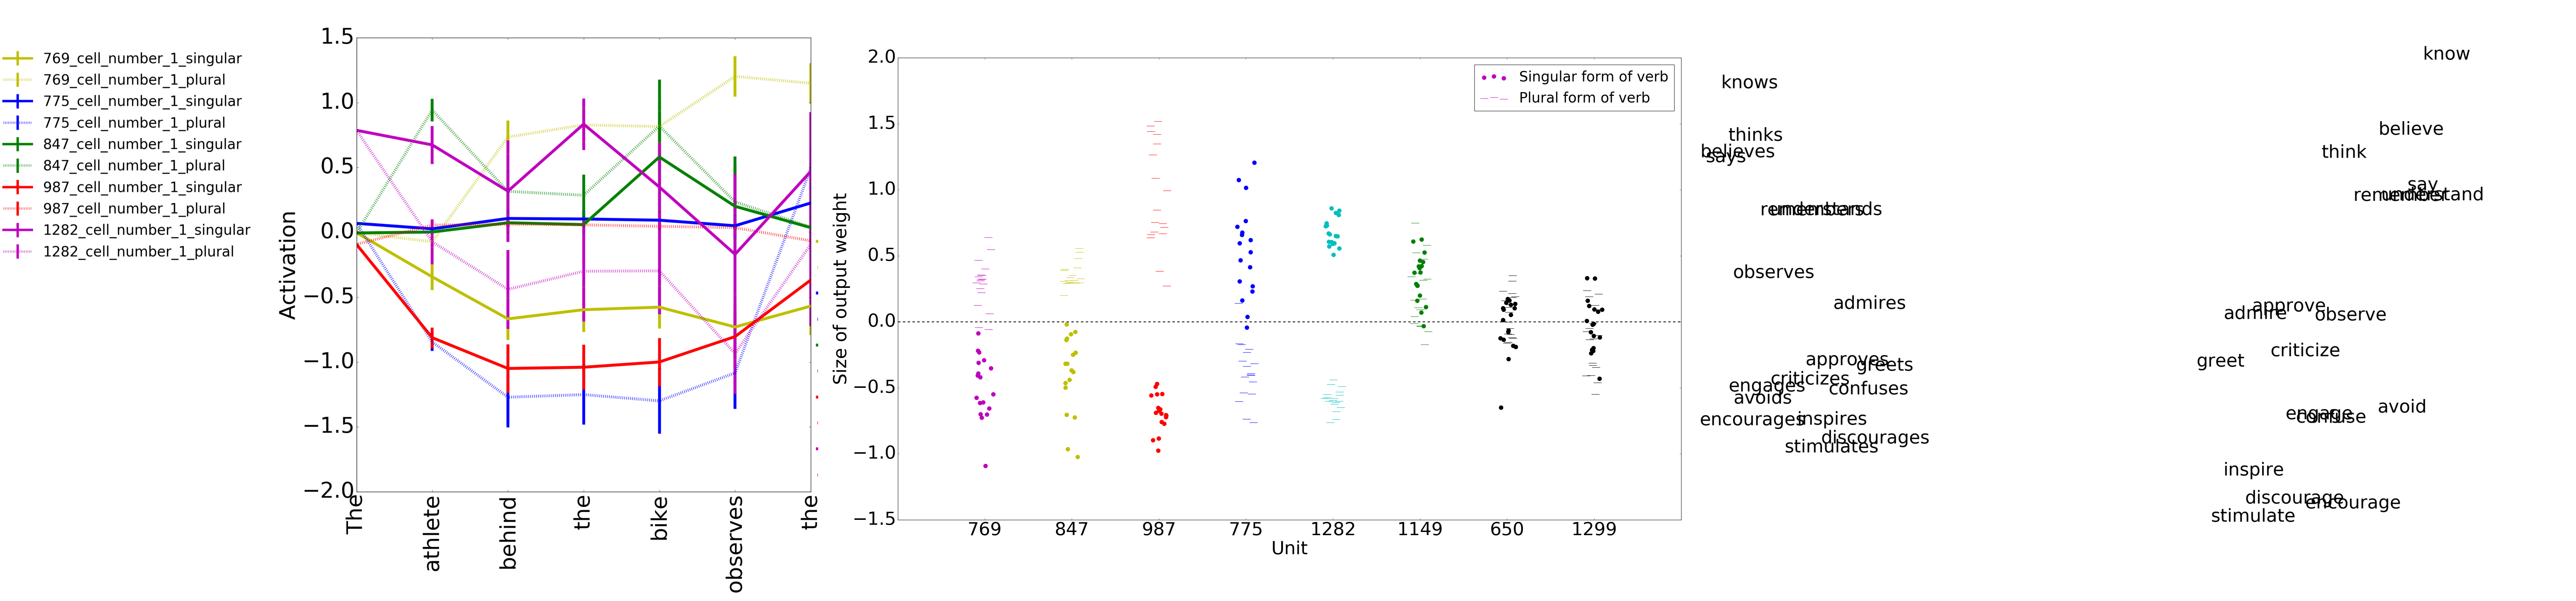
\includegraphics[width=\textwidth]{Figures/Figure4_output_weights.png}
\caption{Connectivity structure to output layer. (A) Output activity $h_t$ of all number units during the processing of a sentence with a PP between subject and verb. (B) Weight values from various units to output layer. Note that only for number units the output weights are clearly separated between singular and plural form of the verb, either positive or negative, compare to the syntax unit (1149) and two non-number units in the second layer. (C) Visualization of 18 verbs in their plural and singular forms (36 words in total) on the plane spanned by the two first principal components of their embeddings by the output weight matrix. A clear separation is observed between the singular and plural form along the first PC.}
\end{figure*}


